\documentclass[a4paper, 12pt]{article}

%%% Работа с русским языком
\usepackage{cmap}					% поиск в PDF
\usepackage{mathtext} 				% русские буквы в формулах
\usepackage[T2A]{fontenc}			% кодировка
\usepackage[utf8]{inputenc}			% кодировка исходного текста
\usepackage[russian]{babel}	% локализация и переносы

%%% Дополнительная работа с математикой
\usepackage{amsmath,amsfonts,amssymb,amsthm,mathtools} % AMS
\usepackage{icomma} % "Умная" запятая: $0,2$ --- число, $0, 2$ --- перечисление

%% Номера формул
%\mathtoolsset{showonlyrefs=true} % Показывать номера только у тех формул, на которые есть \eqref{} в тексте.

%% Шрифты
\usepackage{euscript}	 % Шрифт Евклид
\usepackage{mathrsfs} % Красивый матшрифт

%% Поля
\usepackage[left=2cm,right=2cm,top=2cm,bottom=2cm,bindingoffset=0cm]{geometry}

%% Русские списки
\usepackage{enumitem}
\makeatletter
\AddEnumerateCounter{\asbuk}{\russian@alph}{щ}
\makeatother

%%% Работа с картинками
\usepackage{graphicx}  % Для вставки рисунков
\graphicspath{{images/}{images2/}}  % папки с картинками
\setlength\fboxsep{3pt} % Отступ рамки \fbox{} от рисунка
\setlength\fboxrule{1pt} % Толщина линий рамки \fbox{}
\usepackage{wrapfig} % Обтекание рисунков и таблиц текстом

%%% Работа с таблицами
\usepackage{array,tabularx,tabulary,booktabs} % Дополнительная работа с таблицами
\usepackage{longtable}  % Длинные таблицы
\usepackage{multirow} % Слияние строк в таблице

%% Красная строка
\setlength{\parindent}{2em}

%% Интервалы
\linespread{1}
\usepackage{multirow}

%% TikZ
\usepackage{tikz}
\usetikzlibrary{graphs,graphs.standard}

%% Верхний колонтитул
\usepackage{fancyhdr}
\pagestyle{fancy}

%% Перенос знаков в формулах (по Львовскому)
\newcommand*{\hm}[1]{#1\nobreak\discretionary{}
	{\hbox{$\mathsurround=0pt #1$}}{}}

%% Мои дополнения
\usepackage{float} %Добавляет возможность работы с командой [H] которая улучшает расположение на странице
\usepackage{gensymb} %Красивые градусы
\usepackage{graphicx}               % Импорт изображений
\usepackage{caption} % Пакет для подписей к рисункам, в частности, для работы caption*
\usepackage{indentfirst}


\begin{document}

\newcommand{\HRule}{\rule{\linewidth}{0.7mm}} % Defines a new command for the horizontal lines, change thickness here
	
	\begin{center}
		\large\textbf{Московский Физико-Технический Институт}\\ % Name of your university/college
		\large\textbf{(государственный университет)}
	
		\vfill
		
		\Large Лабораторная работа по курсу общей физики № 4.5.3\\[0.5cm] % Preambule of your document title
		
		
		\HRule
		\\[0.4cm]
		{ \huge \bfseries Сканирующий интерферометр}% Title of your document
		\\[0.4cm] 
		\HRule
		\\[0.5cm]
		
		\ \\
	\textbf{\large Автор:} \\	
	\large Лепарский Роман Б01-003\\ % Your name and something more, your group num for example
		\vfill
		\hspace*{-0.8 cm}
\includegraphics[width=100 pt]{frkt_logo}\\ % logo of your  company/university/college
		\large Долгопрудный, 2022 % location and year
	\end{center}

\newpage
\setcounter{page}{2}
\fancyfoot[c]{\thepage}
\fancyhead[L] {Работа № 4.5.3} % some information in page header
\fancyhead[R]{}
\section{Аннотация}
\textbf{Цель работы:} ознакомление с методами получения и анализа поляризованного света.

\textbf{Приборы и материалы:} оптическая скамья с осветителем, зеленый светофильтр, два поляроида, черное зеркало, полированная эбонитовая пластинка, стопа стеклянных пластинок, слюдяные пластинки разной толщины, пластинки в 1/4 и 1/2 длины волны, пластинка в одну длину волны для зеленого света.

\section{Теоретические сведения}

\subsection{Определение направления разрешённой плоскости колебаний поляроида}

Определить направление разрешённых колебаний поляроида проще всего с помощью чёрного зеркала.

Луч света,
прошедший поляроид и отразившийся от чёрного зеркала, имеет минимальную интенсивность, если: во-первых, свет
падает на отражающую поверхность под углом Брюстера и, во-вторых,
в падающем луче вектор E лежит в плоскости падения.

Измеряя угол поворота зеркала (угол Брюстера), нетрудно определить коэффициент преломления материала, из которого оно изготовлено.

\subsection{Получение эллиптически поляризованного света}
\begin{wrapfigure}{r}{0.35\linewidth} 
	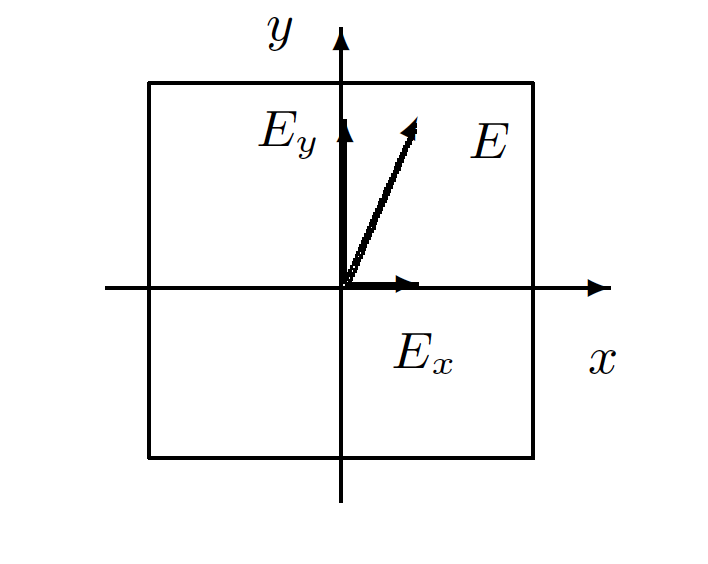
\includegraphics[width=\linewidth]{1}
	\caption{Разложение линейно поляризованного света по главным направлениям двоякопреломляющей пластинки}
	\label{ris 1}
\end{wrapfigure}

Эллиптически поляризованный свет можно получить из линейно поляризованного с
помощью двоякопреломляющих кристаллических пластинок.

Двоякопреломляющая пластинка имеет два взаимно перпендикулярных главных направления. Волны, поляризованные вдоль главных направлений, распространяются в пластинке с разными скоростями, не изменяя характера своей поляризации. Эти волны называются главными. 

Разложим вектор $ \mathbf{E} $ на составляющие $ E_x $ и $ E_y $. На входе пластинки $ E_x $ и $ E_y $ находятся в фазе. На выходе появляется разность хода $ d(n_x - n_y) $, при этом сдвиг фаз определяется соотношением

\begin{equation*}\label{}
\Delta \phi  = k d(n_x - n_y)
\end{equation*}

\begin{wrapfigure}{l}{0.3\linewidth}
	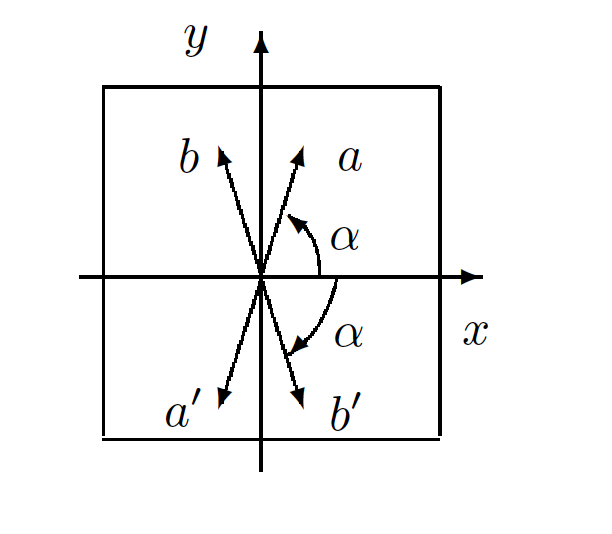
\includegraphics[width=\linewidth]{2}
	\label{ris 2}
\end{wrapfigure}


Рассмотрим практически важные частные случаи.

\begin{enumerate}
	
	\item Пластинка даёт сдвиг фаз $ 2\pi $ (пластинка в длину волны $ \lambda $). В результате сложения волн на выходе пластинки образует-
	ся линейно поляризованная волна с тем же направлением колебаний, что и в падающей волне.
	
	\item Пластинка даёт сдвиг фаз $ \pi $ (пластинка в полдлины волны $ \lambda / 2 $). На выходе пластинки снова образуется линейно поляризованная волна. Направление $ bb' $ колебаний этой волны является отражением направления $ aa' $ колебаний падающей волны (рис. 2).
	
	\item Пластинка создаёт между колебаниями сдвиг фаз $ \pi/2 $ (пластинка
	в четверть длины волны). При сложении двух взаимно перпендикулярных колебаний, имеющих разность фаз $ \pi/2 $, образуется эллипс, главные оси которого совпадают с координатными осями $ x $ и $ y $. При равенстве амплитуд возникает круговая поляризация.
	
\end{enumerate}


\subsection{Анализ эллиптически поляризованного света}

Анализ эллиптически поляризованного света сводится к нахождению главных осей
эллипса поляризации и к определению направления вращения электрического вектора.

Главные оси эллипса поляризации определяются с помощью анализатора по максимуму и минимуму интенсивности проходящего света.
Направление вращения электрического вектора может быть найдено
с помощью пластинки в четверть длины волны, для которой известно,
какая из главных волн, $ E_x $ или $ E_y $, имеет б\'{o}льшую скорость распространения (и соответственно меньшее значение показателя преломления).


\subsection{Пластинка чувствительного оттенка}

\begin{wrapfigure}{l}{0.35\linewidth}
	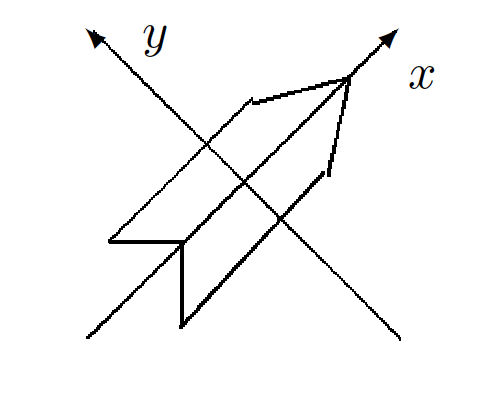
\includegraphics[width=\linewidth]{3}
	\caption{Пластинка
		чувствительного
		оттенка}
	\label{ris 3}
\end{wrapfigure}

Выше предполагалось известным, какому из двух главных направлений пластинки в четверть длины волны соответствует большая скорость распространения света.
Установить это можно различными способами, например с помощью
пластинки чувствительного оттенка.

Пластинка имеет форму стрелы (рис. 3), вдоль оси которой расположено главное направление, соответствующее большей скорости распространения.

Если между скрещенными поляроидами поместить пластинку чувствительного оттенка
($ \lambda $) и пластинку в $ \lambda/4 $ так, чтобы их главные
направления совпадали, цвет пластинки изменится. Если у пластинки чувствительного оттенка и пластинки в $ \lambda/4  $совпадут главные направления, соответствующие большей скорости распространения, то разность хода между $ E_x $ и $ E_y $ для зелёного света составит уже $ 5\lambda/4 $. Это соответствует разности хода в $ \lambda $ для света с большей длиной волны, т. е. для "<более красного"> света. При освещении
этих пластинок (напомним, что они расположены между скрещенными поляроидами) белым светом теперь погасится не зелёная, а красная
часть спектра, и проходящий свет будет казаться зеленовато-голубым.
Если же главные направления, соответствующие большей скорости распространения, у пластинки чувствительного оттенка и у пластинки
в $ \lambda/4 $ окажутся перпендикулярными, то проходящий свет приобретёт
оранжево-желтую окраску (погасится фиолетово-голубая часть спектра).

Изменение цвета позволяет, таким образом, определить, какое из
главных направлений пластинки в $ \lambda/4 $ соответствует большей скорости
распространения.

\subsection{Интерференция поляризованных лучей}

\begin{wrapfigure}{r}{0.35\linewidth}
	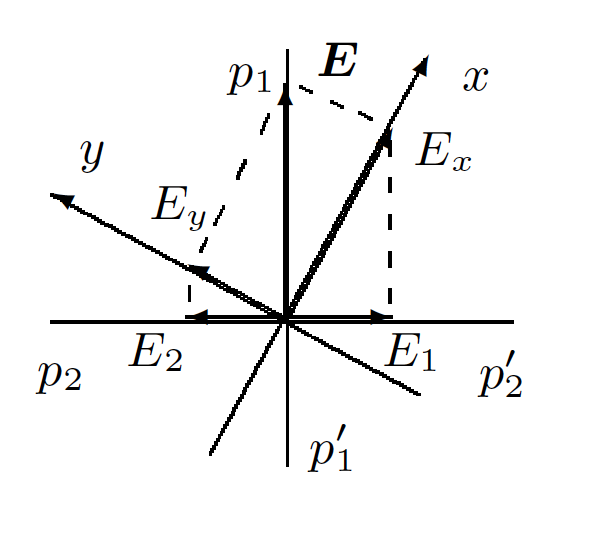
\includegraphics[width=\linewidth]{4}
	\caption{К объяснению интерференции
		поляризованных лучей}
	\label{ris 4}
\end{wrapfigure}


Тонкие двоякопреломляющие пластинки, помещённые между поляроидами, кажутся окрашенными. Эта окраска может быть истолкована как результат интерференции поляризованных лучей. На рис. 4 представлена схема для
случая скрещенных поляроидов.

Здесь $ p_1p'_1 $ --- разрешённое направление колебаний поляризатора
(первого поляроида); $ x, y $ --- координатная система, связанная с главны-
ми направлениями двоякопреломляющей пластинки; $ p_2p'_2 $ --- разрешённое направление колебаний анализатора (второго поляроида). Волны
$ E_x  $ и $ E_y $ на выходе из пластинки когерентны, но не могут интерферировать, так как $ E_x \perp  E_y $. Волны $ E_1 $ и $ E_2 $ на выходе второго поляроида
также являются когерентными и к тому же поляризованы в одной плоскости. Эти волны интерферируют между собой. Результат интерференции определяется зависящим от длины волны сдвигом фаз между $ E_1 $
и $ E_2 $. В результате интерференции поляризованных лучей пластинка, освещаемая белым светом, кажется окрашенной.

Если поворачивать двоякопреломляющую пластинку, расположенную между
скрещенными поляроидами, то соотношение амплитуд волн $ E_1 $ и $ E_2 $ и разность фаз между ними не изменяются. Это означает, что цвет пластинки при её поворотах не меняется, а меняется только интенсивность света. За один оборот пластинки интенсивность четыре раза обращается в нуль --- это происходит при совпадении главных направлений
$ x $ и $ y $ с разрешёнными направлениями колебаний поляроидов.

Если же двоякопреломляющую пластинку оставить неподвижной, а
второй поляроид повернуть так, чтобы разрешённые направления $ p1p'1 $
и $ p2p'2 $ совпали, то волны $ E_1 $ и $ E_2 $ приобретают дополнительный фазовый сдвиг на $ \pi $ для всех спектральных компонент; при этом их амплитуды изменятся так, что цвет пластинки изменится на дополнительный. 

	
\section{Обработка результатов}

	\subsection{Определение разрешенных направлений поляроидов}
Найдем разрешенное направление поляроидов. Для этого поворотом зеркала и поляроида добьемся минимальной интенсивности.

\begin{figure}[H]
	\centering
	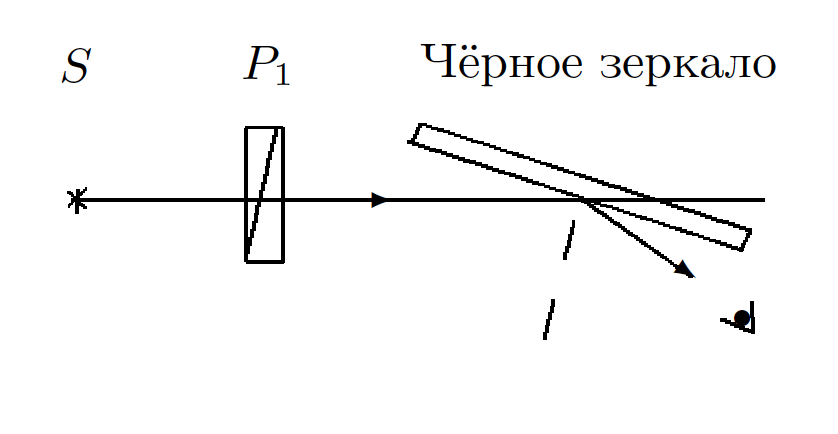
\includegraphics[scale=0.5]{5}
	\caption{Вид сверху}
\end{figure}
Для первого поляроида (здесь и далее разрешенное направление 1-го поляроида ориентированно горизонтально) угол поворота $\alpha_p^1 = 176^\circ\pm2^\circ$.

Определить направление второго поляроида можно так 
\begin{figure}[H]
	\centering
	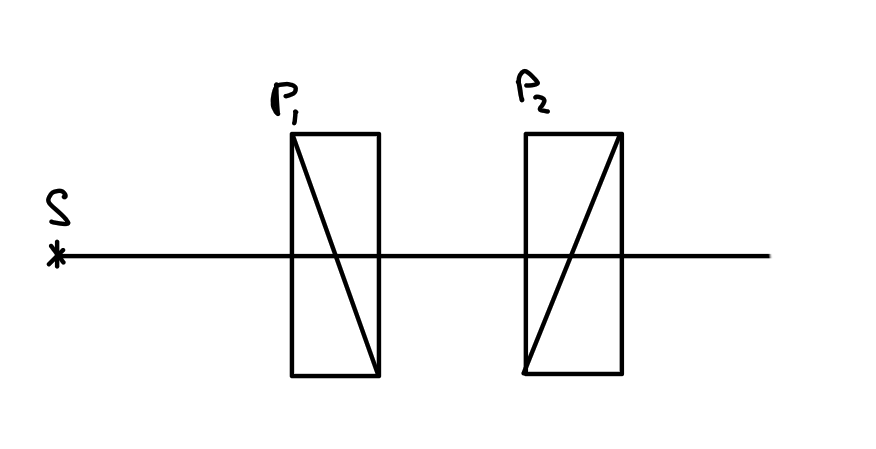
\includegraphics[scale=0.8]{9}
\end{figure}
Интенсивность будет минимальна, если разрешенное направление 2-го поляроида будет перпендикулярно первому. Это происходит при угле $\alpha_p^2=120^\circ\pm1^\circ$.

	\subsection{Определение коэффициента преломления эбонита}
Теперь определим угол Брюстера для эбонита. Воспользуемся схемой аналогичной рис. 4, только в место зеркала расположим эбонитовую пластину. Запишем показания лимба в перпендикулярном положении и под углом Брюстера.
\begin{table}[H]
	\centering
	\begin{tabular}{|c|c|c|}
		\hline
		$\alpha^0$            & $\alpha^1$            & $\varphi_B = \alpha^1-\alpha^0$ \\ \hline
		$179^\circ\pm1^\circ$ & $238^\circ\pm1^\circ$ & $59^\circ\pm1^\circ$            \\ \hline
	\end{tabular}
\end{table}
Для измерений с фильтром результаты оказались теми же.

Показатель преломления $n$ посчитаем так
\[
	n = \tan{\varphi_B} = 1,66\pm0,06
\]
\[
	\sigma_n = \sqrt{\left(\frac{\sigma_{\varphi_B}}{\cos^2{\varphi_B}}\right)^2}
\]
Табличное значение показателя преломления эбонита: $n = 1,6-1,7$.

	\subsection{Определение характера поляризации света в преломленном и отраженном от стопы лучах}
Теперь соберем следующую схему со стопой стеклянных пластин:
\begin{figure}[H]
	\centering
	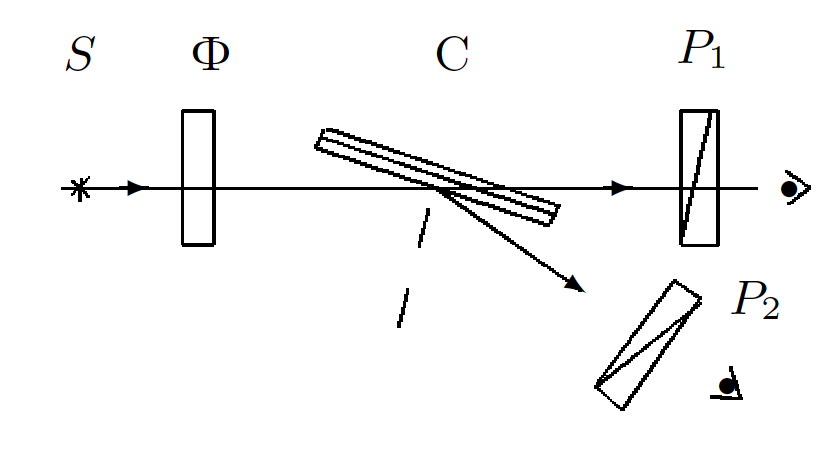
\includegraphics[scale=0.5]{6}
\end{figure}
С помощью поляроида можно увидеть, что отраженный свет имеет вертикальную поляризацию. При рассматривании прошедшего луча, при повороте поляроида заметны перепады яркости, но свет никогда не исчезает полностью. Это значит, что есть не линейно поляризованная составляющая.

	\subsection{Определение главных направлений двоякопреломляющих пластин}

	Расположим пластину между двумя скрещенными поляроидами.
	\begin{figure}[H]
		\centering
		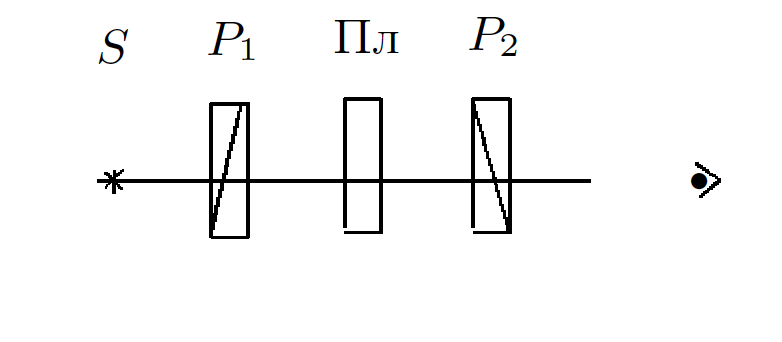
\includegraphics[scale=0.5]{7}
	\end{figure}
	Теперь, вращая пластинку будем наблюдать за минимумами интенсивности прошедшего света. В этом случае главные направления пластинки совпадут с разрешенными направлениями поляроидов.
	
	Пластинка 1:
	\[
		\alpha_1^1 = 110^\circ
	\]
	\[
		\alpha_1^2 = 20^\circ
	\]
	Видно, что направления взаимно перпендикулярны.
	
	Пластинка 2:
	\[
	\alpha_2^1 = 261^\circ
	\]
	\[
	\alpha_2^2 = 171^\circ
	\]
	
	\subsection{Выделение пластин $\lambda/2$ и $\lambda/4$}
	Добавим к предыдущей схеме зеленый фильтр и развернем исследуемую пластинку под $45^\circ$ относительно осей поляроидов. Теперь, вращая анализатор определим характер поляризации.
	
	Пластинка 1: Линейная поляризация, а значит это пластинка $\lambda/2$.
	
	Пластинка 2: Круговая поляризация, а значит это пластинка $\lambda/4$.
	
	\subsection{Определение "быстрой" и "медленной" осей в пластинке $\lambda/4$}
	
	Соберем следующую схему:
	\begin{figure}[H]
		\centering
		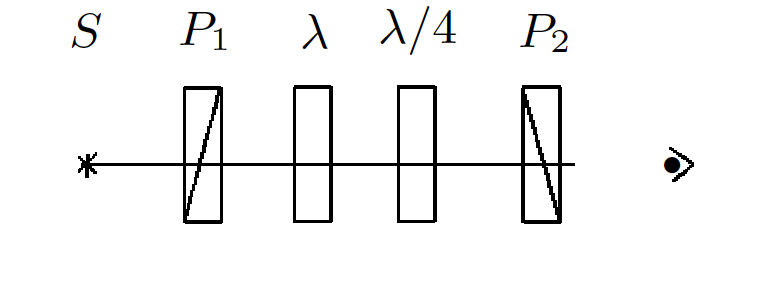
\includegraphics[scale=0.5]{8}
	\end{figure}
	При этом главные оси пластинок повернуты под $45^\circ$. Добавим к этой схеме фильтр. 
	
	Если мы расположим стрелку параллельно оси пластинки, соответствующей углу $\alpha_2^1 = 261^\circ$, то увидим, что она окрасилась в оранжевый цвет. А это значит, что не меняется поляризация синего оттенка $\lambda_b = \dfrac{3}{4}\lambda_g$, то есть $\alpha_2^1 = 261^\circ$ - медленная ось
	
	Теперь повернем стрелку, чтобы она стала параллельна оси $\alpha_2^2 = 171^\circ$. Видно, что цвет стрелки стал голубым. Это означает, что красный свет $\lambda_r = \dfrac{5}{4}\lambda_g$ не изменил поляризацию. Соответственно ось $\alpha_2^2 = 171^\circ$ - быстрая.
	
	\subsection{Интерференция поляризованных лучей}
	Расположим между скрещенными поляроидами мозаичную слюдяную пластинку. При повороте ее относительно поляроидов на $45^\circ$ квадраты окрашиваются в различные цвета. 
	
	Теперь, если мы будем вращать пластинку, будет с периодом $\pi/2$ изменяться интенсивность с сохранением цвета квадратов.
	
	Если же вращать анализатор, у квадратов будет инвертироваться цвет с тем же периодом.
	
	\subsection{Определение направления вращения светового вектора}
		Расположим быструю ось пластинки $\lambda/4$ горизонтально, тогда вышедший свет будет поляризован так:
	\begin{figure}[H]
		\centering
		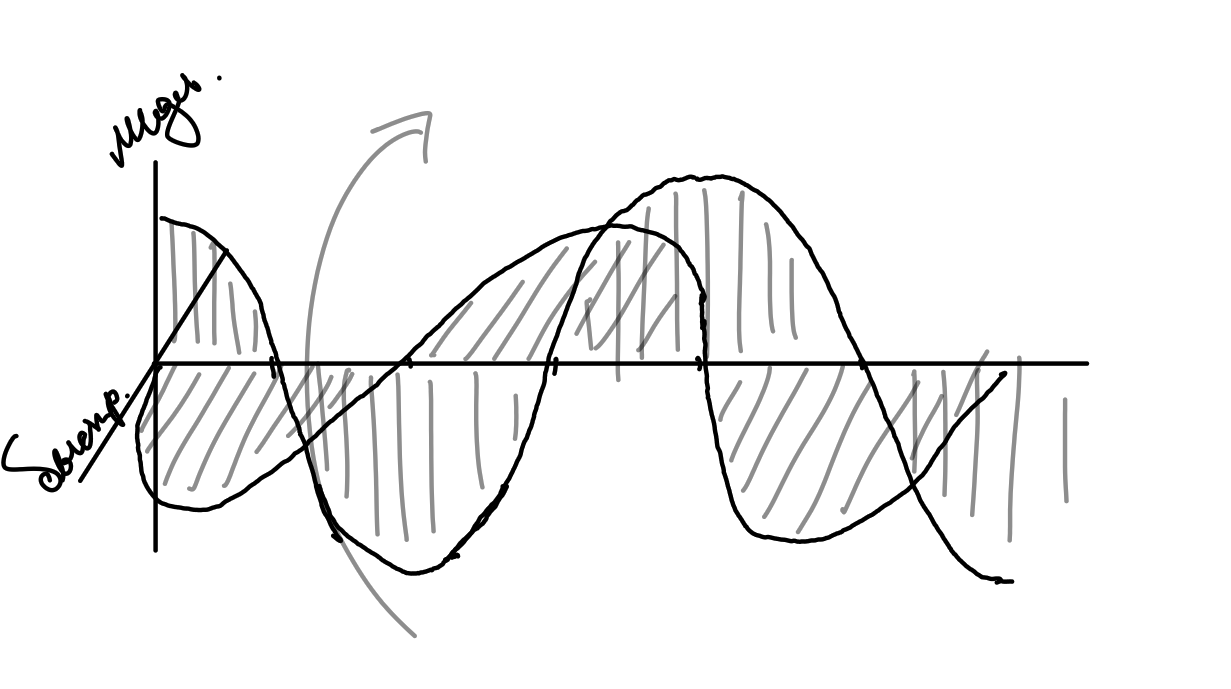
\includegraphics[scale=0.8]{10}
	\end{figure}
	Направление вращения светового вектора - по часовой стрелке.
	
	Пластинку расположим между скрещенными поляроидами, после источника установим фильтр. Теперь, чтобы создать эллиптическую поляризацию, повернем первый поляроид на небольшой угол ($20^\circ$), чтобы световой вектор оказался во 2 и 4 квадрантах. Теперь параллельно нашей пластинке установим другую (тоже $\lambda/4$), у которой заранее определили главные оси.
	
	Теперь, с помощью анализатора определим положение светового вектора. Он находится по прежнему во 2 и 4 квадрантах, а значит пластинки по одиночке дают эллипсы, вращающиеся в разные стороны.
	
\section{Вывод}
	В этой работе мы ознакомились с методами получения и анализа поляризованного света. А так же определили коэффициент преломления эбонита.
	
	
	
	
	
	
	
	
	
	
	
	
	
	
	
	
	
	
	

\end{document}